\chapter{Appendices}

\section{Time Plan}
% \textbf{Time plan}

\begin{table}[H]
  \begin{center}
    \leavevmode
\hangcaption[Semester 1 Time-plan]{Semester 1 Time-plan}
\begin{tabular}{|l|c|c|c|c|c|c|c|c|c|c|c|} \hline
& \multicolumn{11}{c|}{SEMESTER 1} \\ \hline
\rowcolor{white} Week & 1 & 2 & 3 & 4 & 5 & 6 & 7 & 8 & 9 & 10 & 11 \\ \hline
\rowcolor{white} Project Proposal & & \cellcolor{black} & \cellcolor{black} & \cellcolor{black} & & & & & & & \\ \hline
\rowcolor{white} Continuous Presentation & & & & & \cellcolor{black} & \cellcolor{black} & \cellcolor{black} & \cellcolor{black} & \cellcolor{black} & \cellcolor{black} & \cellcolor{black} \\ \hline
\rowcolor{white} Literature Review & & & & & & \cellcolor{black} & \cellcolor{black} & \cellcolor{black} & \cellcolor{black} & \cellcolor{black} & \cellcolor{black} \\ \hline
\rowcolor{white} Mechanical Design & & & & & & & \cellcolor{black} & \cellcolor{black} & \cellcolor{black} & \cellcolor{black} & \\ \hline
\rowcolor{white} Electrical Design & & & & & & & \cellcolor{black} & \cellcolor{black} & \cellcolor{black} & \cellcolor{black} & \\ \hline
\rowcolor{white} Software Design & & & & & & & & & \cellcolor{black} & \cellcolor{black} & \cellcolor{black} \\ \hline
\rowcolor{white} Material Acquisition & & & & & & & & & & & \cellcolor{black} \\ \hline
\end{tabular}
\label{table:semester1timeplan}
\end{center}
\end{table}

\begin{table}[H]
  \begin{center}
    \leavevmode
\hangcaption[Semester 2 Time-plan]{Semester 2 Time-plan}
\begin{tabular}{|l|c|c|c|c|c|c|c|c|c|c|c|c|c|c|} \hline
& \multicolumn{14}{c|}{SEMESTER 2} \\ \hline
\rowcolor{white} Week & 1 & 2 & 3 & 4 & 5 & 6 & 7 & 8 & 9 & 10 & 11 & 12 & 13 & 14 \\ \hline
\rowcolor{white} Continuos Presentation & \cellcolor{black} & \cellcolor{black} & \cellcolor{black} & \cellcolor{black} & \cellcolor{black} & \cellcolor{black} & \cellcolor{black} & \cellcolor{black} & \cellcolor{black} & & & & & \\ \hline
\rowcolor{white} Literature Review & \cellcolor{black} & \cellcolor{black} & \cellcolor{black} & \cellcolor{black} & \cellcolor{black} & & & & & & & & & \\ \hline
\rowcolor{white} Material Acquisition & \cellcolor{black} & \cellcolor{black} & & & & & & & & & & & & \\ \hline
\rowcolor{white} Mechanical Fabrication & & \cellcolor{black} & \cellcolor{black} & \cellcolor{black} & & & & & & & & & & \\ \hline
\rowcolor{white} Electrical Fabrication & & & \cellcolor{black} & \cellcolor{black} & \cellcolor{black} & & & & & & & & & \\ \hline
\rowcolor{white} Software Fabrication & & & & \cellcolor{black} & \cellcolor{black} & \cellcolor{black} & \cellcolor{black} & & & & & & & \\ \hline

\rowcolor{white} Assembly & & & & & & \cellcolor{black} & \cellcolor{black} & \cellcolor{black} & \cellcolor{black} & & & & & \\ \hline
\rowcolor{white} Testing & & & & & & \cellcolor{black} & \cellcolor{black} & \cellcolor{black} & \cellcolor{black} & \cellcolor{black} & \cellcolor{black} & & & \\ \hline
\rowcolor{white} Demonstration & & & & & & & & & & \cellcolor{black} & \cellcolor{black} & \cellcolor{black} & \cellcolor{black} & \cellcolor{black} \\ \hline
\end{tabular}

\label{table:semester2timeplan}
\end{center}
\end{table}


\section{PCB Designs}

\begin{figure}[H]
    \centering
    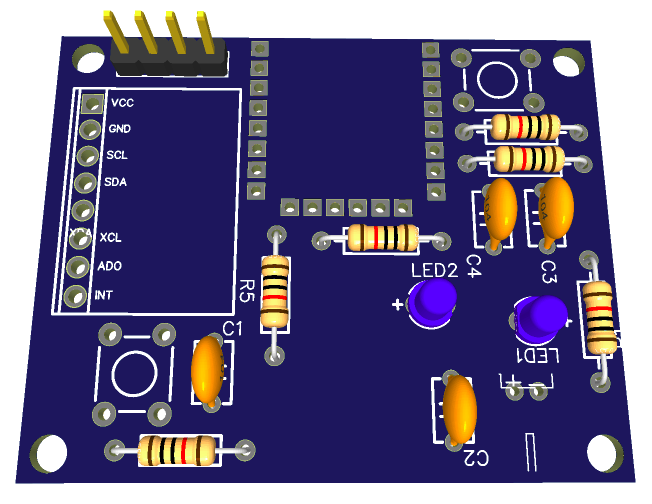
\includegraphics[scale=0.5]{Figures/HMpcb_top.png}
    \caption{Hand Motion Top view of PCB}
    \label{fig:handmotiontopview}
\end{figure}


\begin{figure}[H]
    \centering
    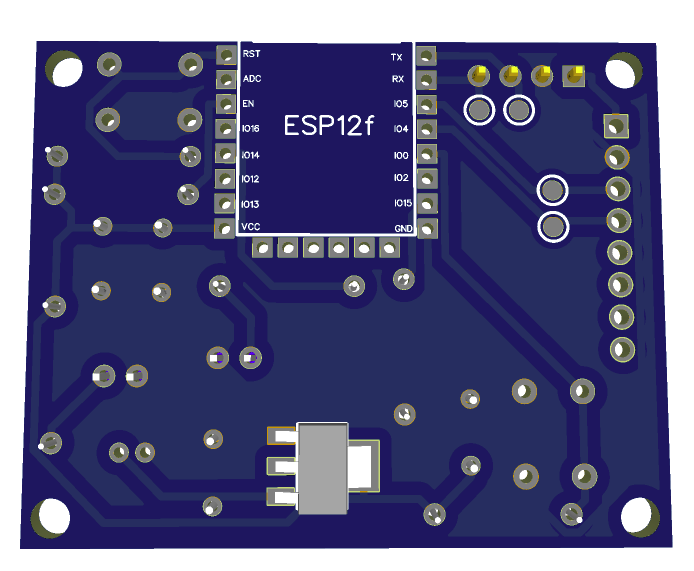
\includegraphics[scale=0.5]{Figures/HMpcb_bottom.png}
    \caption{Hand Motion Bottom view of PCB}
    \label{fig:handmotionbottomview}
\end{figure}


\begin{figure}[H]
    \centering
    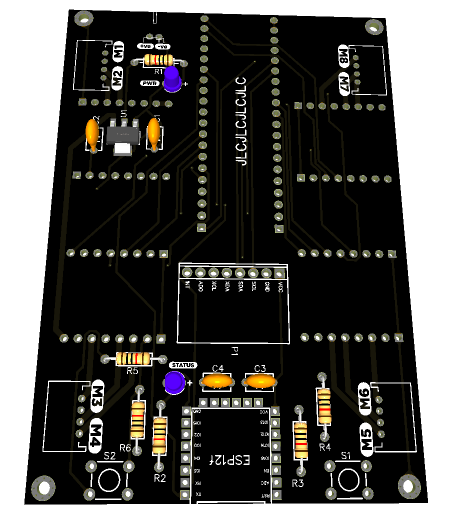
\includegraphics[scale=0.5]{Figures/MPpcb_top.png}
    \caption{Mobile Platform top view}
    \label{fig:mobileplatformtopview}
\end{figure}

\begin{figure}[H]
    \centering
    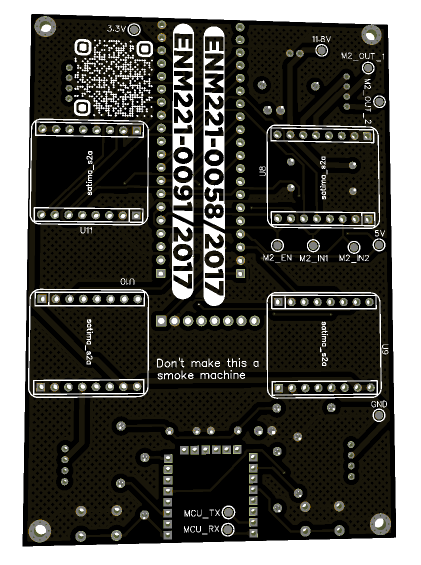
\includegraphics[scale=0.5]{Figures/MPpcb_bottom.png}
    \caption{Mobile Platform bottom view}
    \label{fig:mobileplatformbottomview}
\end{figure}



\section{Production Plans}

\subsection{Mechanical Module}

\begin{enumerate}
    \item Material acquisition. Aluminium sheets to form the platform body and iron rods to construct the chassis will be sourced from a local hardware. Caster wheels will be purchased from an online store.
    \item Once the materials have been acquired, fabrication will commence.
    \item Fabrication techniques to be carried out on the sheet metal that forms the platform body are: sheet metal cutting, sheet metal bending, and boring holes.
    \item The five different parts of the platform will be fabricated using the techniques mentioned above.
    \item Once the different parts have been made, they'll be assembled together using machine screws and nuts.
    \item Fabrication of the chassis will then be conducted by cutting steel rods into the required lengths and joining them using arc welding.
    \item The wheel frames will be fabricated using the same techniques as the parts forming the platform as they are made from sheet metal. 
    \item Once the wheel frames have been made, the motor will be attached using a motor bracket. The wheel and wheel shaft will then be attached allowing the power transmission system of belts and pulley to be attached.
    \item Having assembled the wheel frame components, the frame will be attached to the chassis using a bearing. The platform will then be attached onto the chassis-wheel frame assembly using machine screws.
\end{enumerate}

\subsection{Electrical Module}

\subsubsection{Hand Motion Control PCB}
\begin{enumerate}
    \item Print out the bottom layer onto the Shiny Side of the glossy paper. The copper pads and tracks should be black from figure \ref{fig:HMbottomlayer}.
    \item Sand the copper plate so there is a rough surface for the design to stick to when transferred
    \item Wash the copper with some water and rubbing alcohol and let it dry
    \item Cut out the designs and place them face down on the copper
    \item Run the copper plate with the design face down through a laminator or iron box 5-7 times until the plate is hot 
    \item After running the plate through a laminator or iron place the plate into a cold bath and agitate until the paper floats off
    \item Place the PCB into the etching solution and agitate for 25-30 minutes or until all the copper has dissolved around the design.
    \item Once all the copper is gone rinse it in the water bath, let it dry and use rubbing alcohol to whip off the ink transferred onto the PCB
    \item Drill the holes for DIP components and also mounting holes
    \item Start by placing SMD components and solder them either by hot air gun or hand soldering
    \item Solder DIP components by hand soldering
\end{enumerate}

\begin{figure}[H]
    \centering
    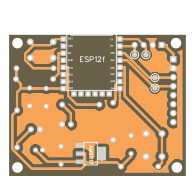
\includegraphics[scale=0.9]{Figures/pcb_bottom.png}
    \caption{Hand motion controller bottom layer}
    \label{fig:HMbottomlayer}
\end{figure}

\subsubsection{Mobile Platform PCB}
For the Mobile Platform PCB it would be great to use using PCB companies such as Gearbox or JLCPCB as it is highly complex for manual fabrication
\begin{enumerate}
    \item Obtain the GitHub repository \cite{gerber_files}.
    \item Submit the Gerber files to respective manufacturer.
\end{enumerate}

\subsection{Software and Control}
The mobile application will be developed using the Flutter framework and Dart language. Flutter applies widgets to construct different features of a window. The basic procedure for Flutter app development is:
\begin{enumerate}
    \item Establish the foundational blocks and classes
    \item Add widgets to the various windows. These widgets can be stateless or stateful widgets depending on whether data/objects change over time.
    \item These widgets are used to add text, images, padding or any other desired frontend features
    \item The application will involve controlling the platform using buttons, so a button widget will be implemented on one window. This widget will be stateful as objects will be changing with time
    \item Once the application has been developed, it will be deployed onto the app stores for the various platforms-android and iOS.
\end{enumerate}